\documentclass[aps,twocolumn,secnumarabic,balancelastpage,amsmath,amssymb,nofootinbib,floatfix]{revtex4-1}

\usepackage{graphicx}      % tools for importing graphics
\usepackage[colorlinks=true]{hyperref}  % this package should be added 
\usepackage{dcolumn}% Align table columns on decimal point
\usepackage{bm}% bold math
\usepackage{xcolor}

\usepackage{tikz}         % tools for drawing figures
\setlength{\parskip}{5pt}
\usetikzlibrary{decorations.pathmorphing}

\newcommand{\keV}{\,{\rm keV}}
\newcommand{\mV}{\,{\rm mV}}
\newcommand{\s}{\,{\rm s}}
\newcommand{\mus}{\,{\rm \mu s}}
\newcommand{\Hz}{\,{\rm Hz}}


\begin{document}

\title{Compton scattering measurement of $661.7\keV$ photons in NaI scintillators}

\author{Vinh Tran}
\affiliation{Department of Physics and Kavli Institute for Astrophysics and Space Research, Massachusetts Institute of Technology, Cambridge, MA 02139, USA}
\email{vinhtran@mit.edu}

\date{\today}

%%%%%%%%%%%%%%%%%%%%%%%%%%%%%%%%%%%%%%%%%%%%%%%%%%%%%%%%%%%%%%%%%%

\begin{abstract}

Compton scattering, long served as a key experiment in the development of quantum mechanics, describes the inelastic scattering of high-energy photons off electrons. In this experiment, we measure the Compton scattering effects of $661.7\keV$ photons from a Cs$^{137}$ source in NaI scintillators using a fairly simple setup. We observe the energy-angle dependency of the scattered photons and recoil electrons, as well as the differential scattering rates of the recoil electrons. The results are consistent with the Compton scattering theory and the Klein-Nishina formula, confirming the validity of the model in this energy regime.

\end{abstract}

\maketitle

%%%%%%%%%%%%%%%%%%%%%%%%%%%%%%%%%%%%%%%%%%%%%%%%%%%%%%%%%%%%%%%%%%

\section{Introduction}
\label{sec:intro}

Compton scattering, first observed by Arthur H. Compton in 1923~\citep{Compton1923}, describes the process where a high-energy photon (often in the X-ray regime) scatters inelastically off a charged particle, typically an electron. The phenomenon served as a foundational experiment in the development of quantum mechanics, playing a key role as experimental evidence for the particle-like behavior of light, requiring both quantum mechanics and special relativity in explaining the change of the photon energy and momentum. Compton scattering has since been used in a variety of applications, including astrophysics~\citep{Birkinshaw1999}, medical imaging, and radiation therapy~\citep{Harding1997}.

Here, we present the measurements of scattering effects between $661.7\keV$ photons from a Cs$^{137}$ source and electrons in NaI scintillators. The experiment was performed using the Compton scattering apparatus at the Junior Lab, Massachusetts Institute of Technology (MIT)~\cite{MIT2023}. We aim to confirm the Compton scattering theory by measuring the energy of the scattered photons and the recoil electrons, as well as determining the differential cross section of the scattering process. In Section \ref{sec:theory}, we present the theoretical background of Compton scattering, focusing on the scattering kinematics, and introduce the differential cross sections in different regimes. Section \ref{sec:experiment} describes the experimental setup and data collection process. Section \ref{sec:analysis} outlines our analysis pipeline for the energy spectrum. In Section \ref{sec:result}, we present the results of the experiment, including the energy-angle dependency and scattering rate. Finally, we discuss the results and conclude in Section \ref{sec:conclusion}.


\section{Inelastic scattering of photon}
\label{sec:theory}

\subsection{Scattering kinematics}
\label{ssec:scattering_kinematics}

\begin{figure}[h]
    \centering
    \vspace{-0.75cm} % Adjust this value as needed to reduce extra space above the figure
    \begin{tikzpicture}[scale=1.5,>=stealth, baseline={(0,0)}]
        % Draw the incident photon arrow (from left to the vertex)
        \draw[decorate, decoration={snake, amplitude=0.5mm, segment length=4mm}, thick, ->] (-2,0) -- (0,0) node[midway, above, inner sep=5] {$\gamma$};
    
        \draw[-, dashed] (0,0) -- (2,0);
    
        % Mark the scattering vertex
        \fill (0,0) circle (1.5pt);
    
        % Draw the recoil electron arrow (at phi=30° above horizontal)
        \draw[->, thick](0,0) -- ({2*cos(-45)},{2*sin(-45)}) node[midway, below, inner sep=10] {$e^-$};
        
        % Draw the scattered photon arrow (at theta=20°)
        \draw[decorate, decoration={snake, amplitude=0.5mm, segment length=4mm}, thick, ->]  (0,0) -- ({2*cos(30)},{2*sin(30)}) node[midway, above, inner sep=10] {$\gamma'$};
    
        % Mark the recoil angle phi (single arc for clarity)
        \draw (0.375,0) arc (0:-45:0.375);
        \draw (0.425,0) arc (0:-45:0.425);
        \node at (0.6,-0.25) {$\phi$};
    
        % Mark the scattering angle theta (double arc from horizontal to electron arrow)
        \draw (0.4,0) arc (0:30:0.4);
        \node at (0.6,0.15) {$\theta$};
    \end{tikzpicture}
    \caption{Compton scattering of a photon by an electron. $\gamma$ and $\gamma'$ are the incident and scattered photons. $e^-$ is the recoil electron initially at rest. $\theta$ and $\phi$ are the scattering and recoil angles, respectively.}
    \label{fig:scattering}
\end{figure}

Following relativistic kinematics, we treat photons as massless particles of energy $E_\gamma = h \nu$, where $h$ is the Planck constant and $\nu$ is the photon frequency. The energy of an electron is given by $E_e = \sqrt{m_e^2 c^4 + p_e^2 c^2}$, where $m_e$ is the electron rest mass, $p_e$ is the electron momentum, and $c$ is the speed of light. By conservation of energy $E$ and momentum $\vec{p}$, we have
\begin{align}
    \label{eq:energy_conservation}
    E_\gamma + E_e &= E_\gamma^{\prime} + E_e^{\prime}, \\
    \label{eq:momentum_conservation}
    \vec{p}_\gamma + \vec{p}_e &= {\vec{p}_\gamma}^{\,\prime} + {\vec{p}_e}^{\,\prime},
\end{align}
where the prime denotes the final state. For simplicity, we take the initial electron energy as $E_e = m_e c^2$, that is, the particle is initially at rest. Solving Equations \eqref{eq:energy_conservation} and \eqref{eq:momentum_conservation}, we obtain the energy of the scattered photon as
\begin{equation}
    \label{eq:scattered_photon_energy}
    E_\gamma^{\prime} = \frac{E_\gamma}{1 + \frac{E_\gamma}{m_e c^2} (1 - \cos \theta)},
\end{equation}
with $\theta$ being the scattering angle, i.e., the angle between the initial and final photon momenta. The kinetic energy of the recoil electron is then calculated as $K_e^{\prime} = E_\gamma - E_\gamma^{\prime}$. The scattering scheme is illustrated in Figure \ref{fig:scattering}.


\subsection{Differential cross section}
\label{ssec:differential_cross_section}

In the classical regime, the differential cross section, defined as the probability of scattering into a solid angle ${\rm{d}}\Omega$, of Compton scattering can be approximated by the Thomson formula for elastic collisions~\citep{Jackson1975}, given by
\begin{equation}
    \label{eq:thomson_cross_section}
    \frac{{\rm{d}}\sigma_{\rm{T}}}{{\rm{d}}\Omega} = r_e^2 \frac{1 + \cos^2{\theta}}{2},
\end{equation}
where $r_e = \frac{e^2}{4 \pi \epsilon_0 m_e c^2}$ is the classical electron radius, with $e$ being the electron charge and $\epsilon_0$ the vacuum permittivity. The Thomson formula remains valid for low-energy photons, i.e., when $E_\gamma \ll m_e c^2$. In more general cases, calculations involving the relativistic quantum mechanism effects of the scattering process are required. The differential cross section is then given by the Klein-Nishina formula~\citep{Weinberg1995}
\begin{equation}
    \label{eq:klein_nishina_cross_section}
    \frac{{\rm{d}}\sigma_{\rm{KN}}}{{\rm{d}}\Omega} = \frac{r_e^2}{2} \left(\frac{\lambda}{\lambda^\prime}\right)^2 \left[\frac{\lambda}{\lambda^\prime} + \frac{\lambda^\prime}{\lambda} - \sin^2{\theta}\right],
\end{equation}
where $\lambda$ and $\lambda^\prime$ are the wavelengths of the incident and scattered photons, respectively.


\section{Experiment setup}
\label{sec:experiment}

\subsection{Apparatus}
\label{ssec:apparatus}

In this experiment, we observe the scattering of $661.7\keV$ photons from a Cs$^{137}$ source off electrons in a NaI scintillator. These electrons, although bound, can be approximated as free electrons due to the high energy of the incident photons. The experimental setup consists of two NaI scintillators, each coupled with a photomultiplier tube (PMT), an amplifier system, and a multichannel analyzer (MCA), consisting of 2048 equally spaced energy channels. The first scintillator functions as the scattering target, while the second is situated at different angles to detect the scattered photons. We denote these instruments as the recoil and scatter scintillators, respectively. The photomultiplier converts the scintillation light into an electrical signal, which is then amplified and processed by the MCA.

To isolate specific scattering events from the background, we employ a coincidence technique, where only events detected within certain time windows ($\tau \simeq 2\mus$) are recorded. Using this setup, background events are typically filtered; however, false detections can still occur, with the rate of
\begin{equation}
    \label{eqn:false_detection_rate}
    n_{\rm{F}} \simeq 2 \tau n_{\rm{r}} n_{\rm{s}},
\end{equation}
where $\tau$ is the aforementioned time window, $n_{\rm{r}}$ and $n_{\rm{s}}$ are the background rates at the recoil and scatter scintillators, respectively. To further reduce such rates, we employ a discriminator circuit, which only allows signals above a certain threshold to pass through. For the setup, we observe a comparable signal rate of $\sim 20\Hz$ across scattering angles in both scintillators. When the Cs$^{137}$ source is blocked, and the threshold is set at $60\mV$, the background rate is reduced to $\lesssim 1\Hz$ in both scintillators for the Compton scattering-relevant channels.

\subsection{Data collection}
\label{ssec:data_collection}

\begin{table}
    \centering
    \addtolength{\tabcolsep}{3pt}
    \def\arraystretch{1.2}
    \begin{tabular}{c c c c}
        \hline
        $\theta$ & Counting Time & Total Time & Collection Date \\ [0ex]
        $[\rm{deg}]$ & $[\rm{s}]$ & $[\rm{s}]$ & [YYYY-MM-DD] \\ [1ex]
        \hline\hline

        0 & 964 & 1012 & 2025-03-04 \\
        30 & 1194 & 1224 & 2025-03-04 \\
        60 & 1619 & 1658 & 2025-03-04 \\
        90 & 1856 & 1900 & 2025-03-04 \\
        120 & 1706 & 1736 & 2025-03-04 \\
        15 & 1354 & 1522 & 2025-03-06 \\
        45 & 1333 & 1455 & 2025-03-06 \\
        75 & 1954 & 2058 & 2025-03-06 \\
        105 & 1645 & 1727 & 2025-03-06 \\
        135 & 1341 & 1431 & 2025-03-06 \\
        
        \hline
        
    \end{tabular}
    \caption{Measurement summary of the Compton scattering experiment. The counting time is the time for which the MCA was collecting data in coincidence mode, while the total time represents the total time the experiment was running. The table does not include the Na$^{22}$ and Ba$^{133}$ calibration measurements of the two scintillators, collected separately on each measuring date.}
    \label{tab:data_collection}    
\end{table}

We perform measurements using the aforementioned setup at $10$ scattering angles. The MCA counting times of each measurement are summarized in Table \ref{tab:data_collection}. These times are chosen to ensure sufficient statistical significance in the count per bin, typically $\sim 30$, corresponding to the signal-noise ratio (SNR) of $\sim 5.5$, for channels neighboring the signal peak. For each measuring date, we include a set of calibration measurements using the Na$^{22}$ source, which displays a distinct electron-positron annihilation peak at $511\keV$, and the Ba$^{133}$ source, which exhibits various clear signatures in the energy spectrum~\citep{Heath1964,Amman2012}. These calibration measurements provide an accurate conversion method from the MCA channel number to energy in keV.

\section{Analysis}
\label{sec:analysis}

\begin{figure}
    \centering
    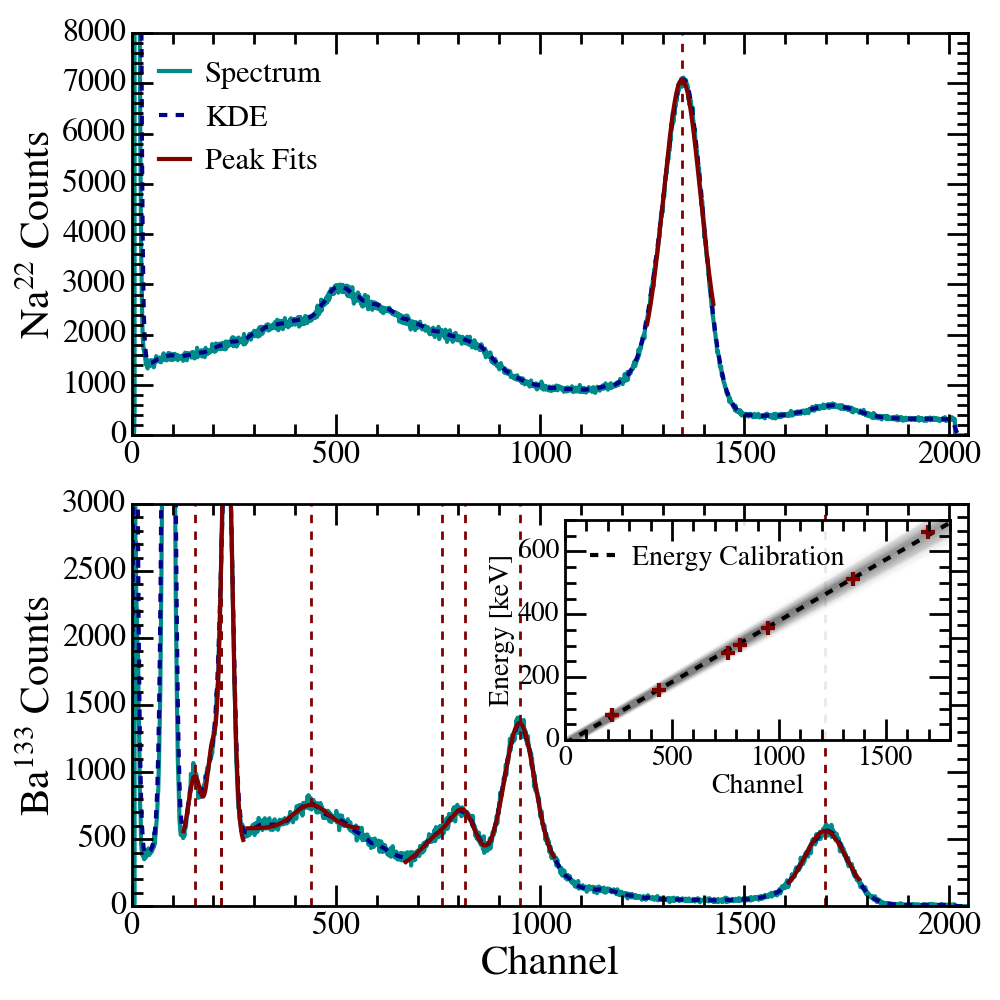
\includegraphics[width=0.49 \textwidth]{Figures/energy_calibration.png}
    \caption{The energy spectra analysis for the calibration measurements of the recoil scintillator on March 4, 2025. The top panel displays the Na$^{22}$ spectrum with the distinct $511\keV$ line, while the bottom panel shows the more populated Ba$^{133}$ spectrum with the additional $661.7\keV$ line from Cs$^{137}$. The blue dashed lines represent the smoothened spectrum, i.e., the Gaussian kernel density estimation (KDE) of the original data (cyan). The sub-panel displays the resulting channel-energy conversion relation (Equation \ref{eq:energy_calibration}) using information from the fitted peaks (dashed red).}
    \label{fig:energy_calibration}
\end{figure}

We follow roughly the same analysis pipeline for the calibration and Compton scattering measurements. For the calibration measurements, as a result of high counting rates, spectra appear smooth, and signature peaks are easily identifiable. The Compton scattering spectra, on the other hand, are more dominated by statistical fluctuations, though relevant peaks remain distinguishable, enabling accurate determination of energies and scattering rates.

In the recoil scintillator, besides the low-energy noise and the incident photon energy peaks, we observe a distinct Gaussian-like feature, corresponding to the energy of the recoiled electron. In the scatter scintillator, the situation is more complicated, with the scattered photon energy peak being accompanied by an additional Compton spectrum. While the scattered energy can still be extracted, the Compton spectrum complicates the measurement of the scattering rate. As a result, we rely primarily on the recoil scintillator for such information.

The analysis pipeline is as follows:
\begin{itemize}
    \item A Gaussian filter (with $\sigma = 5$ channels) is applied to the raw data, smoothing out the noise while preserving the signal peaks.
    \item Local maxima and minima are then identified using derivative-based peak finding algorithm, with close extrema grouped, accounting for statistical fluctuations. These features guide the fitting range and initial guesses. Typically, we limit the fitting range to half or one third maximum with respect to the peak height, unless nearby valleys are more prominent.
    \item Peaks of interest are then fitted using Gaussian functions with optional constant offsets. In the case of calibration measurements, for nearby peaks, we also use triple-peak Gaussian functions to account for the overlapping features. For the Compton scattering measurements, the fittings are performed using a Poisson-based likelihood approach, with the residual sum of squares approximated as
    \begin{multline}
        \hspace{0.75cm} \chi^2 \simeq -\sum_i 2 \left[ y_i \log{\left( \hat{y}_i \right)} - \hat{y}_i - \log{\left( y_i! \right)}\right] \\ 
        + \log{\left(2 \pi y_i\right)},
    \end{multline}
    where $y_i$ and $\hat{y}_i$ are the observed and expected count for the channel $i$, respectively.
    \item The central channel and width of the fitted peaks, along with their uncertainties, are then extracted. For the recoil scintillator, the scattering rate are determined by integrating within the FWHM of the fitted Gaussian, and uncertainties are propagated via Monte Carlo simulations.
\end{itemize}

From the extracted information in the calibration measurements, we obtain the channel-energy conversion relation\footnote{As the triple-peak Gaussian fittings are not optimal, especially for the smaller peaks embedded in larger ones, we limit the linear regression of the channel-energy conversion to peaks with reconstructed error of $< 5\%$.}
\begin{equation}
    \label{eq:energy_calibration}
    E_i = \alpha C_i + b,
\end{equation}
with $E_i$ as the energy corresponding to the channel $C_i$. Here, $\alpha$ and $b$ are the energy scale and offset, respectively. The exact values of $\alpha$ and $b$ depend on the scintillator and measuring date; nevertheless, as per our design, the values are typically similar. Figure \ref{fig:energy_calibration} shows the peak fitting analysis and the channel-energy conversion for the recoil scintillator measured on March 4, 2025. Here, the conversion parameters take the values of $\alpha = 0.390 \pm 0.014\keV$ and $b = -10.5 \pm 6.2\keV$. The uncertainties here, as well as the offset, are systematics in nature. However, for the following analysis, we propagate them as part of the statistical uncertainties.


\section{Results}
\label{sec:result}

\subsection{Energy-angle dependency}
\label{ssec:energy_angle_dependency}

\begin{figure}
    \centering
    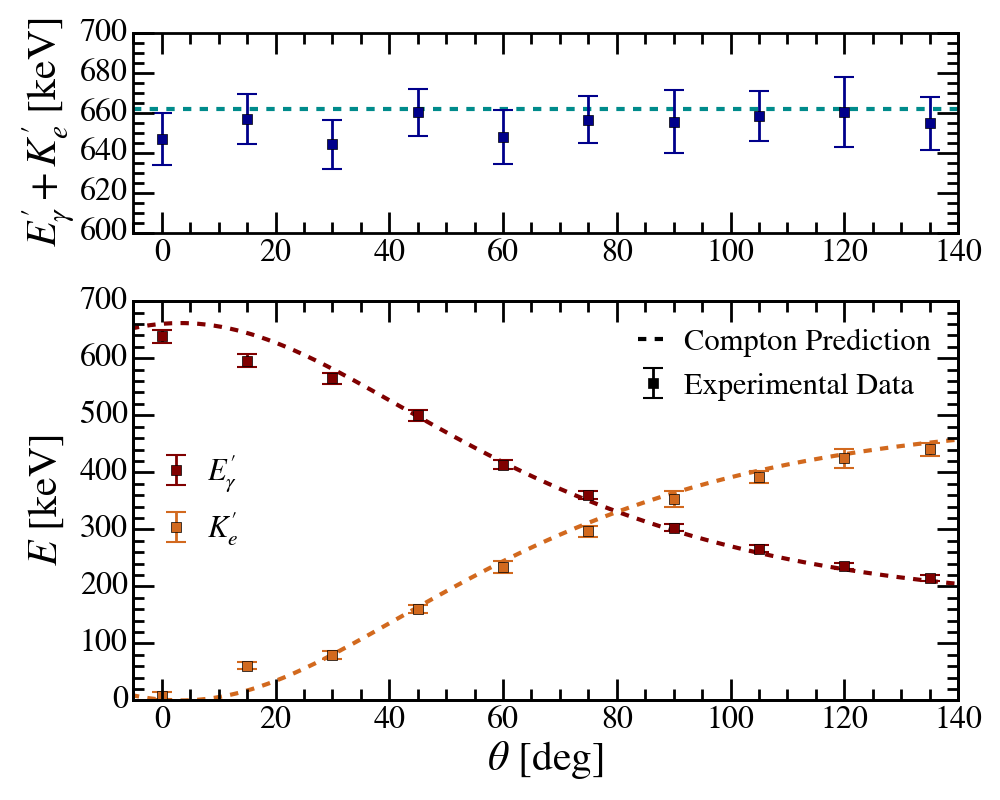
\includegraphics[width=0.49 \textwidth]{Figures/energy_angle_dependency.png}
    \caption{Top: The reconstructed energy of the incident photons at different scattering angles. The cyan dashed line indicates the expected value of $661.7\keV$. Bottom: The energy of the scattered photons $E_\gamma^{\prime}$ (red) and the recoil electrons $K_e^{\prime}$ (orange) as functions of the scattering angle $\theta$. The dashed lines represent the expected values of $E_\gamma^{\prime}$ and $K_e^{\prime}$ according to the theory of Compton scattering. These lines are shifted in respond to the initial offset angle of the system $\theta_0 = 2.56 \pm 0.71^\circ$.}
    \label{fig:energy_angle_dependency}
\end{figure}

Figure \ref{fig:energy_angle_dependency} shows the reconstructed energies of the incident photons $E_\gamma$, scattered photons $E_\gamma^{\prime}$, and recoil electrons $K_e^{\prime}$ as functions of the scattering angle $\theta$\footnote{We note that the errors displayed are the results of fitting uncertainties rather than the widths of the signal peaks. The former represent the uncertainties in the central energies, while the latter signify the spread in energies, which can be the results of various effects, such as the broadening and beam size of the initial Cs$^{137}$ lines, as well as the physical size of the scintillators.}. We observe that $E_\gamma$ remains consistent with the expected value of $661.7\keV$, while the scattered photon energies $E_\gamma^{\prime}$ and $K_e^{\prime}$ exhibit a clear dependency on the scattering angle as predicted by the Compton scattering theory. The values of $E_\gamma$ are typically $\sim 10\keV$ lower than the expected value, which can be attributed to systematic offsets in the scattered photon peaks, the fittings of which are complicated by the presence of the additional Compton spectrum. Additionally, systematic errors arise from the limited arrangement in our apparatus, namely, the offset angle $\theta_0$ of the system, which is not perfectly aligned with the incident photon beam. This angle is estimated using the energy-angle dependency of the recoil electron and take the value of $\theta_0 = 2.56 \pm 0.71^\circ$, the uncertainty of which is equivalent to the systematic error in the scattering angle measurements $\sigma_\theta^{\rm{sys}} \sim 0.5^\circ$.

\subsection{Scattering rate}
\label{ssec:scattering_rate}

\begin{figure}
    \centering
    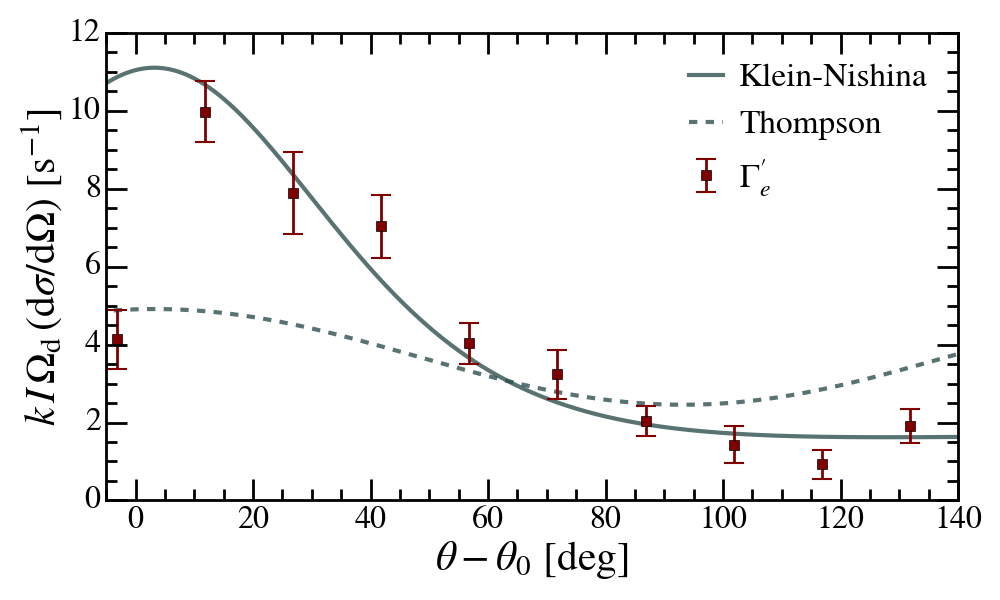
\includegraphics[width=0.49 \textwidth]{Figures/scattering_rate.png}
    \caption{The scaled differential scattering rate of the recoil electrons as a function of the adjusted scattering angle $\theta - \theta_0$. The solid and dashed lines represent the fitted Klein-Nishina and Thomson differential cross sections, respectively. The error bars and shaded regions represent the statistical and systematic uncertainties, respectively.}
    \label{fig:scattering_rate}
\end{figure}

Figure \ref{fig:scattering_rate} shows the scaled differential scattering rate of the recoil electrons as a function of the adjusted scattering angle $\theta - \theta_0$. The scattering rates obtained in Section \ref{sec:analysis} depend linearly on the differential scattering rates though the beam intensity $I$, detector angular size $\Omega_{\rm{d}}$, and the order of unity scaling factor $k$. We observe that for our energy regime, the scattering rates are poorly described by the classical Thomson differential cross section, and a quantum relativistic treatment is required. The Klein-Nishina differential cross section, as expected, provides a better description to the observed scattering rates, with the exception at $\theta = 0^\circ$, where the scintillator and MCA are not sensitive enough to make accurate measurements for low-energy electrons. The formula performs especially well when the systematic uncertainties are taken into account. These uncertainties estimated using the smoothened spectrum of the recoil scintillator, where the uncertainties in the half maximum width of the signal peaks are propagated from variations within the kernel width, are significantly larger than the statistical uncertainties propagated from the fitting errors.


\section{Discussion \& conclusion}
\label{sec:conclusion}

In this experiment, we measure the Compton scattering effects using a simple setup comprising of two NaI scintillators and a Cs$^{137}$ source. We observe the scattering of $661.7\keV$ photons from the recoil electrons in the recoil scintillator, and the scattered photons in the scatter scintillator. The energy-angle dependency of the scattered photons and recoil electrons is consistent with the Compton scattering theory, with the inferred system offset angle of $\theta_0 = 2.56 \pm 0.71^\circ$. The differential scattering rates of the recoil electrons are also consistent with the Klein-Nishina differential cross section, while the Thomson formula fails to describe the data.

The experiment demonstrates the validity of the Compton scattering theory and the Klein-Nishina formula in the energy regime of $661.7\keV$ photons. Even with a relatively simple setup, where energy spectra are dominated by statistical fluctuations, the results remain highly consistent with the theoretical predictions. Future improvements could include a more precise alignment of the apparatus to reduce the systematic uncertainties, as well as the use of better shielding to reduce the background rates.

\begin{acknowledgments}

The author thanks his lab partner Y. Hu for collaboration in the experiment. The author also thanks the JLab teaching staffs S. Patel and C. Romanov for their guidance and support, as well as the MIT Physics Department for providing the experimental apparatus.

\end{acknowledgments}

%%%%%%%%%%%%%%%%%%%%%%%%%%%%%%%%%%%%%%%%%%%%%%%%%%%%%%%%%%%%%%%%%%

\bibliography{ref}

%%%%%%%%%%%%%%%%%%%%%%%%%%%%%%%%%%%%%%%%%%%%%%%%%%%%%%%%%%%%%%%%%%

\end{document}